\chapter{Grundlagen}
% Hier müssen noch die ganzen Referenzen bzw. Quellen eingefügt werden!
In diesem Kapitel wird auf die mathematischen Grundlagen zum Verständnis der Arbeit eingegangen. Während in Abschnitt \ref{sec:Fourierreihen und Fouriertransformation} auf die Darstellung periodischer Funktionen mittels Fourierreihen eingegangen wird, behandelt Abschnitt \ref{sec.Diskrete Fouriertransformation} die mathematische Formulierung der diskreten Fouriertransformation für abgetastete Signale und geht des Weiteren auf das Nyquist-Shannon-Abtasttheorem ein.\\
In Abschnitt \ref{sec.Wahrscheinlichkeitsverteilungen} folgt dann eine Erläuterung zu Wahrscheinlichkeitsverteilungen. Den Anfang bildet hier die Binomialverteilung (Abschnitt \ref{sec.Binomialverteilung}), bevor zuletzt die Poisson-Verteilung (Abschnitt \ref{sec.Poissonverteilung}) besprochen wird.

\section{Fourierreihen und Fouriertransformation}
% Quelle: Eichler 2006
\label{sec:Fourierreihen und Fouriertransformation}
Periodische Signale tauchen in vielen Bereichen der Physik und Technik auf. Ein Signal bezeichnet hierbei eine Funktion, welche eine physikalische Größe in Abhängigkeit von der Zeit, dem Ort, oder einer anderen Variablen darstellt. Betrachtet man periodische Funktionen, so zeichnen sich diese durch ihre Periodendauer $T$ aus. Die gesamten Informationen des Signals stecken in dieser Periode, so dass gilt: $F(t) = F(t+T)$. Jede periodische Funktion kann durch eine Überlagerung von Sinus- und Kosinusfunktionen unterschiedlicher Periodendauern $2 \pi n$ approximiert werden. Dargestellt werden kann dies durch eine Fourierreihe. 

\begin{equation}
	\label{eq:Fourierreihe}
	F(t) = \dfrac{a_0}{2} + \sum_{n=0}^N[a_n \cos(n \omega t) + b_n \sin(n \omega t)]
\end{equation}
Hierbei bezeichnet $\omega = 2 \pi / T$ die Kreisfrequenz der Grundschwingung. Im Allgemeinen geht $N$ gegen $\infty$. Die Konstanten $a_0,a_1 \dots $ werden als gerade Fourierkoeffizienten bezeichnet, $b_1, b_2 \dots $ hingegen als ungerade Fourierkoeffizienten. Dies leitet sich daraus ab, dass der $\cos(x)$ eine gerade und der $\sin(x)$ eine ungerade Funktion ist. \\
Des Weiteren lässt sich eine Fourierreihe durch Sinusfunktionen mit unterschiedlichen Amplituden und Phasen beschreiben. Die Fourierreihe lautet dann:
\begin{equation}
	\label{eq:Fourierreihe_umgerechnet}
	F(t) = \rho_0 + \sum_{n=1}^{N} \rho_n \sin(n \omega t + \Phi_n)
\end{equation}
Die Grundfrequenz des Signals besitzt eine Frequenz $f_1 = 1/ T = \omega / 2 \pi$. Die weiteren Sinus- und Kosinusfunktionen der Fourierreihe besitzen Frequenzen $f_n = nf_1$, also ganzzahlige Vielfache der Grundfrequenz. Die Umrechnung von Gleichung \ref{eq:Fourierreihe} nach Gleichung \ref{eq:Fourierreihe_umgerechnet} erfolgt mithilfe der Definitionen:
\begin{equation}
	\label{eq:rho_0}
	\rho_0 = \frac{a_0}{2}
\end{equation}
\begin{equation}
	\label{eq:rho_n}
	\rho_n = \sqrt{a_n^2 + b_n^2}
\end{equation}
\begin{equation}
	\label{eq:phi_n}
	\Phi_n = \arctan(\frac{a_n}{b_n})
\end{equation}
Mit $\rho_0$ \ref{eq:rho_0} wird hierbei der Gleichanteil des Signals bezeichnet, $\rho_n$ \ref{eq:rho_n} steht für die Amplitude der \textit{n-ten} Frequenz und $\Phi_n$ \ref{eq:phi_n} für die Phasenverschiebung der \textit{n-ten} Frequenz. Ein Signal kann also durch sein Kosinus- und Sinusspektrum sowie durch sein Amplituden- und Phasenspektrum charakterisiert werden. 
% hier muss jetzt noch das Bild 52.1 eingefügt werden, welches das zeitliche Signal beschreibt, sowie Bild 52.2 mit dem Amplituden-und Phasenspektrum. Dann noch Erläuterungen dazu machen.
Grafisch veranschaulicht wird die Fourierreihe durch \bild{Fourier}. Im linken Bild eingezeichnet ist ein periodisches Signal mit der Periodendauer T, für welches also $F(t) = F(t+T)$ gilt. Im rechten Bild finden sich die das Gesamtsignal definierenden Frequenzen, mit ihren zugehörigen Amplituden $\rho$ und Phasenversatz $\Phi$.
\begin{figure}[!ht]
	\centering
	\subfigure[]{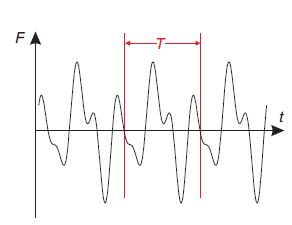
\includegraphics[height=50mm]{signal}}
	\hspace{5mm}
	\subfigure[]{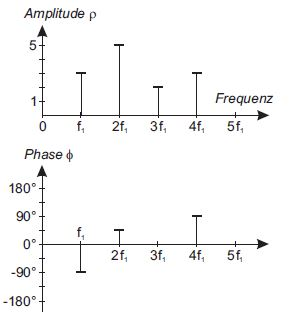
\includegraphics[height=50mm]{amplituden_phasenspektrum}}
	\caption{Periodisches Signal mit zugehörigem Amplituden- und Phasenspektrum (Quelle: Eichler))}
	\label{fig.Fourier}
\end{figure}
\\
Die Fouriertransformation überführt die Gleichung aus dem Zeitbereich $F(t)$ nun in den Frequenzbereich $F(\omega)$. Für analoge Signale ist die Fouriertransformation nun wie folgt definiert:
\begin{equation}
	\label{eq:Fouriertransformation}
	F(\omega) = \int\limits_{-\infty}^{\infty} x(t) e^\ind{-j\omega} \ind{d}t.
\end{equation}
\begin{equation}
	\label{eq:Inverse_Fouriertransformation}
	F(t) = \frac{1}{2\pi}\int\limits_{-\infty}^{\infty} F(\omega)e^\ind{j\omega} \ind{d}\omega
\end{equation}
Gleichung \ref{eq:Fouriertransformation} überführt eine von der Zeit abhängige Funktion aus dem Zeitbereich über Integration von $-\infty$ bis $\infty$ über alle Zeitpunkte $t$ in den Frequenzbereich. Die inverse Fouriertransformation wird durch Gleichung \ref{eq:Inverse_Fouriertransformation} beschrieben. Die Rücktransformation erfolgt durch Integration von $-\infty$ bis $\infty$ des von der Frequenz $\omega$ abhängigen Signals über alle Frequenzen $\omega$.

\section{Diskrete Fouriertransformation}
\label{sec.Diskrete Fouriertransformation}
% Quelle: Wendemuth
Die in Abschnitt \ref{sec:Fourierreihen und Fouriertransformation} dargestellten Gleichungen gelten für analoge Funktionen. In der Praxis ist es aber so, dass keine vollständige Kenntnis über ein Signal vorliegt, sondern dies nur durch Messungen zu diskreten Zeitpunkten abgetastet werden kann. Hieraus resultiert die Diskrete Fourier-Transformation (DFT). Die resultierenden Werte $F(n)$ der diskreten Fouriertransformation eines zu den Zeitpunkten $k$ abgetasteten Signals $f(t)$ können mittels Gleichung \ref{eq:DFT} berechnet werden. Die inverse diskrete Fouriertransformation erfolgt dann durch Gleichung \ref{eq:IDFT}.
\begin{equation}
	\label{eq:DFT}
	F(n) = \sum_{k=0}^{N-1}x[k]e^\ind{j\frac{2\pi}{N}kn}
\end{equation}
\begin{equation}
	\label{eq:IDFT}
	f[k] = \frac{1}{N}\sum_{k=0}^{N-1}F(n)e^\ind{j\frac{2\pi}{N}kn}
\end{equation} \\
Im Zusammenhang mit der Diskreten Fouriertransformation ist abschließend das Abtasttheorem von Nyquist und Shannon zu nennen. Das Theorem besagt, dass ein beliebig geformtes, kontinuierliches Signal immer dann durch ein diskretes Signal darstellbar und auch exakt wiederherstellbar ist, wenn die Abtastfrequenz des Signals mindestens doppelt so hoch ist, wie die höchste im kontinuierlichen Signal enthaltene Frequenz. Beträgt die höchste Frequenz in unserem Signal also beispielsweise \SI{10}{\Hz}, so müssen wir unser Signal mit mindestens \SI{20}{\Hz} abtasten, um unser Signal vollständig rekonstruieren zu können. \\
Die Folgen einer zu geringen Abtastfrequenz werden in \bild{Abtasttheorem} ersichtlich. Die Abtastung des Signals zu den mit schwarz markierten Zeitpunkten reicht nicht aus, um das in grau dargestellte Originalsignal zu rekonstruieren. Stattdessen ergibt sich das in rot dargestellte Signal.
\begin{figure}[!ht]
	\begin{center}
		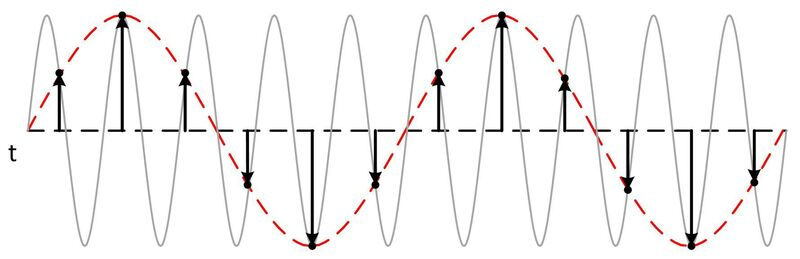
\includegraphics[height=50mm]{abtasttheorem}
		\caption{Originalsignal (grau) und durch Abtastung rekonstruiertes Signal (rot) Quelle(https://www.geothermie.de/bibliothek/lexikon-der-geothermie/a/abtasttheorem.html)}
		\label{fig.Abtasttheorem}
	\end{center}
\end{figure}
\section{Wahrscheinlichkeitsverteilungen}
\label{sec.Wahrscheinlichkeitsverteilungen}
\subsection{Binomialverteilung}
\label{sec.Binomialverteilung}
% Quelle: Teschl 2010
Als Bernoulli-Experiment wird ein Zufallsexperiment bezeichnet, bei dem es lediglich zwei Ausgänge geben kann. Ein Ereignis A tritt entweder ein oder nicht. Führt man ein Bernoulli-Experiment n-mal hintereinander unter den gleichen Bedingungen durch, so erhält man eine Bernoulli-Kette der Länge $n$. Das Eintreten des Ereignisses A wird gemeinhin als Erfolg bezeichnet, die Wahrscheinlichkeit $P(A)=p$ bezeichnet man als Erfolgswahrscheinlichkeit. Als Ereignis A kann hier beispielhaft das Werfen einer Münze mit dem Ausgang $Zahl$ genannt werden. Eine Binomialverteilung entsteht nun, wenn wir die Anzahl der Erfolge bei einer Bernoulli-Kette ermitteln wollen. Mathematisch formuliert lässt sich die Binomialverteilung ausdrücken als:
\begin{equation}
	\label{eq:Binomialverteilung}
	P(X=x) = \binom{n}{x}p^\ind{x} q^\ind{n-x}
\end{equation}\\
$X$ bezeichnet hierbei die Anzahl der Versuchsdurchführungen, bei denen ein Erfolg eintritt. $X$ kann die Werte $x = 0,1,2,\dots,n$ annehmen. $p$ steht für die Eintrittswahrscheinlichkeit eines Erfolges, $q$ für die Wahrscheinlichkeit eines Misserfolges. Die Zufallsvariable $X$ ist binomialverteilt und ihre Wahrscheinlichkeitsverteilung eine Binomialverteilung mit den Parametern $n,p$. Kurz: $X~Bi(n;p)$. Die grafische Darstellung einer Binomialverteilung für die Wahrscheinlichkeit der Anzahl an Würfen eines Würfels mit dem Ereignis 1 bei sieben Würfen ist in Abbildung xy abgebildet.
% Hier Bild aus Buch 2014 Mathe für Informatiker einfügen
% evtl noch Eigenschaften der Binomialverteilung einfügen? Oder unnötig?
\subsection{Poissonverteilung}
\label{sec.Poissonverteilung}
Eine Zufallsvariable $X$, welche unendlich viele Werte $x=0,1,2\dots$ mit den Wahrscheinlichkeiten
\begin{align}
	P(X=x) &= \frac{\lambda^\ind{x}}{x!} e^\ind{-\lambda} & (\lambda >0)
	\label{eq:Poisson Verteilung}
\end{align}
annehmen kann, wird als poissonverteilt mit dem Parameter $\lambda$ bezeichnet. Die zugehörige Verteilung heißt Poisson-Verteilung. Der Erwartungswert sowie die Varianz der Poisson-Verteilung werden ausgedrückt als:
\begin{align}
	\mu &= E(X) = \lambda \\
	\sigma^2 &= Var(X) = \lambda
	\label{eq:Poisson EW und Var}
\end{align}
Anhand der obigen Formeln erkennt man, dass der Parameter der Poisson-Verteilung grade gleich ihres Erwartungswertes ist, selbiges gilt für die Varianz.
Häufig ist es von Interesse, die Anzahl $X_t$ eines Ereignisses innerhalb eines Zeitraumes von 0 bis $t$ zu prognostizieren. Die Menge von Zufallsvariablen $X_t, t\geq 0,$ wird als Poisson-Prozess mit der Intensität $\lambda$ bezeichnet, falls $X_t$ einer Poisson-Verteilung folgt, es also gilt: \\
\begin{equation}
	P(X_t=x) = \frac{(\lambda t)^x}{x!} e^\ind{-\lambda t}
	\label{eq:Poisson-Prozess}
\end{equation}
Ein Poisson-Prozess muss dabei drei Voraussetzungen erfüllen:
\begin{itemize}
	\item Die Wahrscheinlichkeit für ein Ereignis ist proportional zur Beobachtungsdauer $\Delta t$, aber unabhängig von der Lage der Beobachtungsdauer.
	\item Die Wahrscheinlichkeiten für ein Ereignis an unterschiedlichen Orten sind voneinander unabhängig
	\item Für infinitesimal kleine $\Delta t$ ist die Wahrscheinlichkeit, dass das Ereignis mehr als einmal auftritt, im Vergleich zur Wahrscheinlichkeit, dass es genau einmal vorkommt, vernachlässigbar klein.
\end{itemize}

% Vllt noch eine Sektion zu GMM's (Gaussian Mixture Models) ? Wird in Paper Krajnik.2015b aufgegriffen. Evtl. Erklärung da etwas zu kurz gegriffen.


